On considère le cube ABCDEFGH représenté ci-dessous.
	
	\begin{center}
		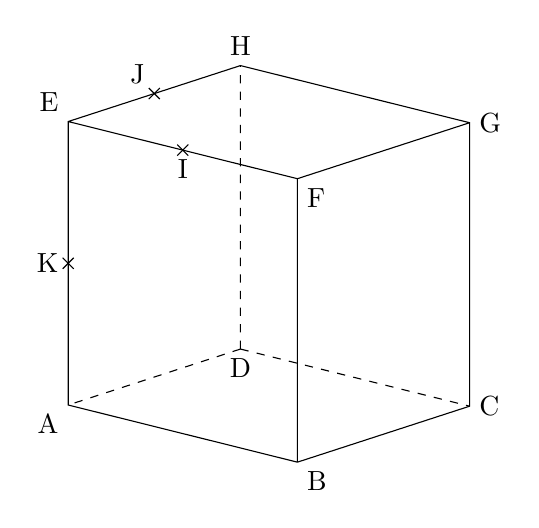
\begin{tikzpicture}[x=(-14:30mm),y=(18:23mm),z=(90:36mm)]
			\draw (0,0,0)node[below left]{A}--
			(1,0,0)node[below right]{B}--
			(1,1,0)node[right]{C}--
			(1,1,1)node[right]{G}--
			(0,1,1)node[above]{H}--
			(0,0,1)node[above left]{E}-- cycle
			(0,0,1) --(1,0,1)node[below right]{F}--(1,0,0)
			(1,0,1) -- (1,1,1);
			\draw[dashed] (0,1,0)node[below]{D}--(0,0,0)
			(0,1,0)--(0,1,1) (0,1,0)--(1,1,0);
			\foreach \coord/\lettre/\pos in {{(0.5,0,1)}/I/{below},{(0,0.5,1)}/J/{above left},{(0,0,0.5)}/K/{left}}
			{\draw[shift={\coord}] (2pt,2pt)--(-2pt,-2pt) (2pt,-2pt)--(-2pt,2pt) (0,0)node[\pos]{\lettre} ;}
		\end{tikzpicture}
	\end{center}
	
	On munit l'espace du repère orthonormal $\left(\mathrm{A};\vectt{AB},\vectt{AD},\vectt{AE}\right)$.
	
	Soit I le milieu du segment [EF], J le milieu de [EH] et K le milieu de [AE].
	
	\begin{enumerate}
		\item Donner les coordonnées des points I, J et K.
		
		\item \begin{enumerate}
			\item Déterminer la valeur du produit scalaire $\vectt{AI}\cdot\vectt{AJ}$.
			
			\item En déduire la mesure de l'angle $\widehat{\mathrm{IAJ}}$ arrondie au dixième de degré.
		\end{enumerate}
		
		\item \begin{enumerate}
			\item Démontrer que le vecteur $\vectt{KC}$ est un vecteur normal au plan (AIJ).
			
			\item En déduire qu'une équation cartésienne du plan (AIJ) est \quad  \[x+y-\dfrac{1}{2}z=0\]
		\end{enumerate}
		
		\item Soit L le projeté orthogonal du point C sur le plan (AIJ).
		\begin{enumerate}
			\item Déterminer les coordonnées du point L.
			
			\item En déduire que la distance du point C au plan (AIJ) est égale à $\dfrac{4}{3}$.
		\end{enumerate}
		
		\item Soit M un point de la droite (FG).
		
		On admet que les coordonnées de M sont $(1 ; m ; 1)$ avec $m$ appartenant à $\R$.
		
		\begin{enumerate}
			\item Démontrer qu'une représentation paramétrique de la droite (IM) est
			\[\begin{cases}
				x=\dfrac{1}{2} s+\dfrac{1}{2} \\
				y=m s \\
				z=1
			\end{cases} \quad \text{avec } s \in \R\]
			
			\item Peut-on affirmer que les droites (IM) et (KC) sont coplanaires quelle que soit la valeur de $m$ ?
		\end{enumerate}
	\end{enumerate}
